
%% bare_conf.tex
%% V1.3
%% 2007/01/11
%% by Michael Shell
%% See:
%% http://www.michaelshell.org/
%% for current contact information.
%%
%% This is a skeleton file demonstrating the use of IEEEtran.cls
%% (requires IEEEtran.cls version 1.7 or later) with an IEEE conference paper.
%%
%% Support sites:
%% http://www.michaelshell.org/tex/ieeetran/
%% http://www.ctan.org/tex-archive/macros/latex/contrib/IEEEtran/
%% and
%% http://www.ieee.org/

%%*************************************************************************
%% Legal Notice:
%% This code is offered as-is without any warranty either expressed or
%% implied; without even the implied warranty of MERCHANTABILITY or
%% FITNESS FOR A PARTICULAR PURPOSE! 
%% User assumes all risk.
%% In no event shall IEEE or any contributor to this code be liable for
%% any damages or losses, including, but not limited to, incidental,
%% consequential, or any other damages, resulting from the use or misuse
%% of any information contained here.
%%
%% All comments are the opinions of their respective authors and are not
%% necessarily endorsed by the IEEE.
%%
%% This work is distributed under the LaTeX Project Public License (LPPL)
%% ( http://www.latex-project.org/ ) version 1.3, and may be freely used,
%% distributed and modified. A copy of the LPPL, version 1.3, is included
%% in the base LaTeX documentation of all distributions of LaTeX released
%% 2003/12/01 or later.
%% Retain all contribution notices and credits.
%% ** Modified files should be clearly indicated as such, including  **
%% ** renaming them and changing author support contact information. **
%%
%% File list of work: IEEEtran.cls, IEEEtran_HOWTO.pdf, bare_adv.tex,
%%                    bare_conf.tex, bare_jrnl.tex, bare_jrnl_compsoc.tex
%%*************************************************************************


\documentclass[conference,onecolumn]{IEEEtran}
\usepackage{blindtext, graphicx}
\graphicspath{ {imgs/} }

% *** GRAPHICS RELATED PACKAGES ***
%
\ifCLASSINFOpdf
  % \usepackage[pdftex]{graphicx}
  % declare the path(s) where your graphic files are
  % \graphicspath{{../pdf/}{../jpeg/}}
  % and their extensions so you won't have to specify these with
  % every instance of \includegraphics
  % \DeclareGraphicsExtensions{.pdf,.jpeg,.png}
\else
  % or other class option (dvipsone, dvipdf, if not using dvips). graphicx
  % will default to the driver specified in the system graphics.cfg if no
  % driver is specified.
  % \usepackage[dvips]{graphicx}
  % declare the path(s) where your graphic files are
  % \graphicspath{{../eps/}}
  % and their extensions so you won't have to specify these with
  % every instance of \includegraphics
  % \DeclareGraphicsExtensions{.eps}
\fi

\hyphenation{op-tical net-works semi-conduc-tor}


\begin{document}

\title{Forecasting CPU usage of Virtual Machines}
\author{\IEEEauthorblockN{Sai Narsi Reddy Donthi Reddy}
\IEEEauthorblockA{School of Electrical and\\Computer Engineering\\
University of Missouri -  Kansas City\\
Email: sdhy7@mail.umkc.edu}}

\maketitle

\IEEEpeerreviewmaketitle



\section{Introduction}
\label{sec:intro}
In this paper we forecast CPU usage by five different virtual machines by using different such as moving average (MA), weighted moving average (WMA), exponential Smoothing(ES), and exponential Smoothing with trend (EST). Along with these basic methods, we also tested moving window regression models.

To test the performance of the forecasting methods we used tracking signal ratio (TS). Tracking signal is the ratio of cumulative sum of forecasting signals to the mean absolute deviation. Which indicates the presents of bias in the results produced by the forecast model.

\begin{equation}
TS = \frac{\sum A_t - F_t}{MAD}
\end{equation}

Where $A_t$ is the actual value, $F_t$ is predicted value and MAD is the mean absolute deviation.

\begin{equation}
MAD = \frac{\sum |A_t - F_t|}{n}
\end{equation}

For a better forecasting model, TS should be not grater than 4 and not less than -4.
\begin{equation}
-4 < TS < +4 
\end{equation}

If tracking signal value is out the limits, then the forecasting model should be re-evaluated. If the TS above 4, most of our predictions as above actual values and vice verse.


\section{Forecasting Techniques}
\label{sec:FT}

\subsection{Moving Average (MA)}
\label{subsec:MA}
In this technique, the forecasting is done by taking the simple average of last n data. i.e., to predict at time $t$ we take the mean of values from $t-n$ to $t-1$ as shown in the equal below.

\begin{equation}
F_t  =  \frac{\sum_{i=1}^{n} A_{(t-i)+1}}{n}, n\leq d
\end{equation}
Where, $F_t$ is the predicted value, $A_t$ are the actual values and window size $n$ should be less than or equal to the total size of the data $d$.

As this is a simple averaging of last $n$ values, this method is computationally simple. However, if there is a lot of variation in the data, this method lags behind the data and produces lot of deviation.

In this paper to test the performance of the moving average method we choose window sizes of $\left \{ 3, 5, 9, 11, 20\right \}$.

\subsection{Weighted Moving Average (WMA)}
\label{subsec:WMA}
Similar to moving average technique, in this method we predict using the last n values. But, instead of given same weights to all the values we assign different weights based on the effect of value will be on the final prediction. In this method one thing to note is that the sum of all the weights should be equal to 1.

\begin{equation}
F_t  =  \sum_{i=1}^{n} W_i * A_{(t-i)+1}, n\leq d
\end{equation}
Where, $F_t$ is the predicted value, $W_i$ are the weights whose some equals to 1 ($\sum_{i=1}^{n} W_i = 1$), $A_t$ are the actual values and window size $n$ should be less than or equal to the total size of the data $d$.

Performance of this method mainly depends on the weights and window parameters. In this paper, as CPU utilization data is collected every 5 min, if the utilization increases there is steep increase or vice verse. So, it is better to have more weight to the latest value in time series than to the old value. To test the performance we use same window sizes as above and for weight simple linear increments is used. i.e., if the window size is $5$ then weights are assigned as $\left \{ \frac{1}{1},\frac{1}{2},\frac{1}{3},\frac{1}{4},\frac{1}{5}\right \}$.

\subsection{Exponential Smoothing (ES)}
\label{subsec:ES}
In exponential smoothing the weight to the past predictions is given in exponentially decreasing manner. Unlike moving average method, where all the n values get equal weights, this method gives exponentially reducing weights and discounted the past data in a more gradual manner \cite{ES}.

If $a$ is the smoothing constant, $F_t$ and $A_t$ are predicted and actual values, then exponential smoothing is given as:

\begin{equation}
F_t = a * A_{t-1} + (1 - a) * F_{t-1}
\end{equation}

To test the performance of this method we use $a$ values of $\left \{ 0.2,0.4,0.6,0.8\right \}$. If $a$ value is close to 1, then more weight is given to the latest actual value and less weight to the last predicted value. Exponential smoothing produces the results by taking interpolation between latest actual value and last predicted value \cite{ES}.

\subsection{Exponential Smoothing with Trend (EST)}
\label{subsec:EST}
The main disadvantage of exponential smoothing (ES) is that it does not follow the trend \cite{ES2}. To overcome this double exponential smoothing or exponential smoothing with trend (EST) is proposed.

If $FIT_t$ is the predicted value with trend, $T_t$ is the trend for current predicting, then exponential smoothing with trend is given as:

\begin{equation}
FIT_t = F_t + T_t
\end{equation}
\begin{equation}
F_t = a * A_{t-1} + (1 - a) * FIT_{t-1}
\end{equation}
\begin{equation}
T_t = T_{t-1} + d (F_t - FIT_{t-1})
\end{equation}
Where, $a$ and $b$ are the prediction smoothing and trend smoothing constants.

For performance testing of exponential smoothing with trend same $a$ values are used and $d = 0.5$.
\subsection{Moving Window Regression (MWR)}
\label{subsec:MWR}
Regression is statistical technique used to estimate the relation among variables \cite{MWR}. This method follows the same technique as moving average, instead of taking the average of the values in given window we fit a polynomial line and predict the value.

To test the performance of the moving window regression, same window sizes as moving average are selected and $1^{st}$ (linear regression) and $2^{nd}$ order polynomial equations are used. 

\section{Experiments}
\label{sec:Experiments}

\subsection{Dataset}
\label{subsec:data}
The CPU utilization data is collected from UMKC datacenter at an intervals of $5min$ for total of $506$ virtual machines. For each virtual machine CPU utilization(MHz) is collect at $5 min$ intervals for $24 hrs$, generating average of 284 values. For the evaluation purpose instead of considering all the virtual machines only 5 are considered randomly.

\begin{figure}[ht]
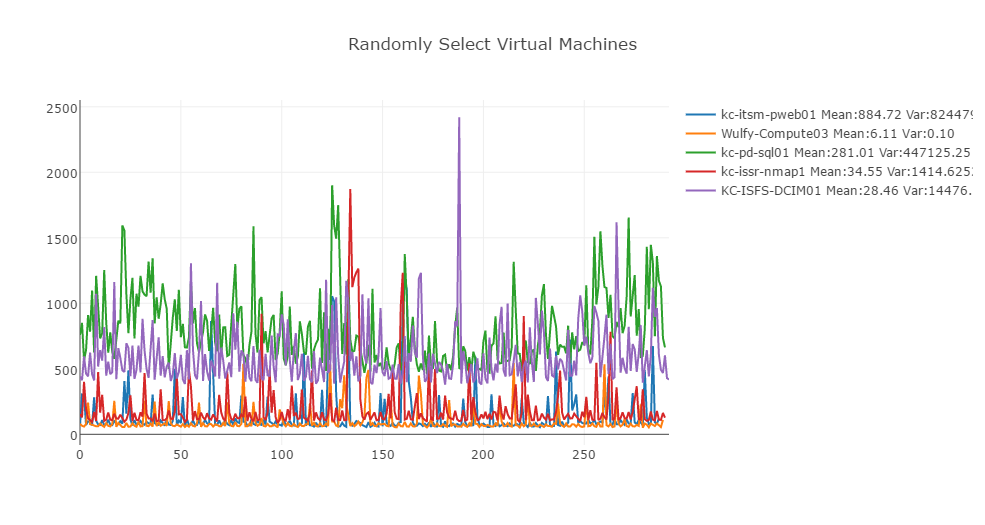
\includegraphics[scale=0.4]{sel_vms}
\centering
\caption{Randomly selected virtual machines, their mean and variance}
\label{fig:sel_vm}
\end{figure}

From Figure - \ref{fig:sel_vm}, it can seen that except virtual machine $Wulfy-Compute03$ all the other virtual machines have very high variance, which results in constantly varying values and predicting these virtual machine CPU utilization will be really difficult.

The performance of each forecasting method is tested using mean absolute deviation (MAD) and tracking signal ratio (TS) as explained in section-\ref{sec:intro}. For the forecasting method to perform better its mean absolute deviation should be close to zero and its tracking signal to be between -4 and +4.


\begin{figure}[ht]
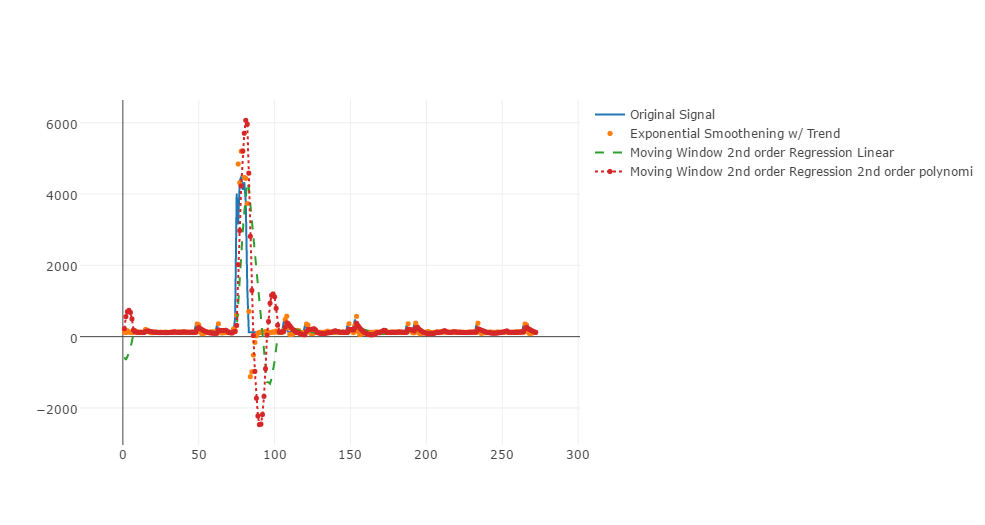
\includegraphics[scale=0.4]{comp}
\centering
\caption{Large trend effect on prediton using exponential smoothong with trend, moving window regression methods.}
\label{fig:comp}
\end{figure}

\subsection{Results}
\label{subsec:results}

\begin{table}[ht]
\centering
\begin{tabular}{|c|c|c|c|c|c|c|c|c|c|c|}
\hline
            & \multicolumn{2}{c|}{kc-itsm-pweb01} & \multicolumn{2}{c|}{Wulfy-Compute03} & \multicolumn{2}{c|}{kc-pd-sql01} & \multicolumn{2}{c|}{kc-issr-nmap1} & \multicolumn{2}{c|}{KC-ISFS-DCIM01} \\ \hline
\multicolumn{11}{|c|}{Moving Average}                                                                                                                                                                  \\ \hline
Window Size & TS               & MAD              & TS                 & MAD             & TS              & MAD            & TS               & MAD             & TS               & MAD              \\ \hline
3.00        & -6.60            & 315.62           & -2.24              & 0.15            & -41.76          & 99.40          & -0.06            & 20.81           & 0.00             & 16.95            \\ \hline
5.00        & -3.89            & 318.02           & -7.76              & 0.15            & -48.52          & 135.29         & 0.25             & 21.31           & 0.08             & 20.50            \\ \hline
9.00        & -11.69           & 336.98           & -8.12              & 0.16            & -30.82          & 175.56         & 0.70             & 21.48           & 0.08             & 26.13            \\ \hline
11.00       & -16.02           & 338.30           & -6.39              & 0.17            & -23.61          & 184.84         & -0.96            & 20.04           & 0.10             & 27.73            \\ \hline
20.00       & -19.29           & 358.36           & -1.58              & 0.19            & -11.14          & 207.24         & 1.06             & 21.14           & 0.10             & 31.58            \\ \hline
\multicolumn{11}{|c|}{Weighted Moving Average}                                                                                                                                                         \\ \hline
Window Size & TS               & MAD              & TS                 & MAD             & TS              & MAD            & TS               & MAD             & TS               & MAD              \\ \hline
3.00        & -6.25            & 314.91           & -1.15              & 0.14            & -41.61          & 85.99          & -0.07            & 20.31           & -0.02            & 14.62            \\ \hline
5.00        & -2.04            & 308.93           & -7.22              & 0.15            & -47.22          & 110.18         & 0.16             & 20.72           & 0.07             & 17.41            \\ \hline
9.00        & -9.05            & 313.74           & -5.33              & 0.15            & -22.32          & 135.49         & 0.33             & 21.18           & 0.07             & 21.68            \\ \hline
11.00       & -12.09           & 316.24           & -3.54              & 0.16            & -13.95          & 145.53         & -1.42            & 20.82           & 0.09             & 23.61            \\ \hline
20.00       & -12.37           & 331.37           & -0.43              & 0.18            & -3.19           & 177.61         & 0.50             & 20.90           & 0.10             & 28.70            \\ \hline
\multicolumn{11}{|c|}{Exponential Smoothing}                                                                                                                                                           \\ \hline
a value     & TS               & MAD              & TS                 & MAD             & TS              & MAD            & TS               & MAD             & TS               & MAD              \\ \hline
0.20        & -17.70           & 325.31           & -28.29             & 0.18            & -33.86          & 173.62         & 1.02             & 19.93           & 0.19             & 21.90            \\ \hline
0.40        & -8.70            & 311.55           & -16.01             & 0.16            & -25.43          & 116.54         & 0.20             & 19.93           & 0.08             & 16.60            \\ \hline
0.60        & -5.83            & 319.04           & -11.17             & 0.15            & -22.27          & 88.89          & 0.06             & 19.77           & 0.05             & 13.45            \\ \hline
0.80        & -4.64            & 336.73           & -8.52              & 0.15            & -19.75          & 75.11          & 0.01             & 19.75           & 0.02             & 11.26            \\ \hline
\multicolumn{11}{|c|}{Exponential Smoothing with Trend}                                                                                                                                                \\ \hline
a value     & TS               & MAD              & TS                 & MAD             & TS              & MAD            & TS               & MAD             & TS               & MAD              \\ \hline
0.20        & 5.16             & 373.62           & 0.32               & 0.21            & -0.63           & 255.11         & -0.30            & 25.80           & 1.86             & 34.66            \\ \hline
0.40        & 0.81             & 358.03           & 0.16               & 0.19            & -0.25           & 152.81         & -0.31            & 27.27           & -0.03            & 20.14            \\ \hline
0.60        & -0.19            & 373.95           & -0.01              & 0.18            & 0.04            & 114.20         & -0.10            & 26.17           & -0.06            & 15.24            \\ \hline
0.80        & -1.11            & 405.86           & 0.00               & 0.19            & 0.04            & 98.42          & -0.11            & 25.99           & -0.07            & 14.80            \\ \hline
\multicolumn{11}{|c|}{Moving window Regression 1st order polynomial}                                                                                                                                   \\ \hline
Window Size & TS               & MAD              & TS                 & MAD             & TS              & MAD            & TS               & MAD             & TS               & MAD              \\ \hline
3.00        & -2.92            & 479.21           & 3.11               & 0.21            & -7.17           & 99.59          & -0.07            & 32.39           & -0.12            & 16.03            \\ \hline
5.00        & 3.91             & 384.22           & -3.24              & 0.19            & -3.91           & 112.45         & -0.13            & 29.46           & 0.01             & 17.06            \\ \hline
9.00        & 0.57             & 334.49           & 3.26               & 0.18            & 24.87           & 142.35         & -0.52            & 28.43           & -0.02            & 22.77            \\ \hline
11.00       & 0.96             & 341.35           & 4.62               & 0.18            & 25.04           & 161.19         & -2.04            & 27.58           & 0.03             & 26.29            \\ \hline
20.00       & 7.46             & 323.71           & 2.23               & 0.20            & 16.32           & 212.39         & -0.74            & 23.82           & 0.05             & 34.56            \\ \hline
\multicolumn{11}{|c|}{Moving window Regression 2nd order polynomial}                                                                                                                                   \\ \hline
Window Size & TS               & MAD              & TS                 & MAD             & TS              & MAD            & TS               & MAD             & TS               & MAD              \\ \hline
3.00        & -2.10            & 1124.95          & -1.80              & 0.56            & 5.29            & 198.19         & -0.05            & 73.65           & -0.09            & 23.23            \\ \hline
5.00        & -0.82            & 599.81           & -5.10              & 0.31            & 4.61            & 138.66         & -0.03            & 47.43           & 0.08             & 21.20            \\ \hline
9.00        & -1.78            & 416.08           & 3.30               & 0.23            & 13.10           & 138.94         & 0.21             & 37.86           & -0.13            & 24.52            \\ \hline
11.00       & 0.19             & 381.49           & 1.60               & 0.23            & 0.63            & 153.50         & 0.01             & 34.34           & -0.07            & 26.34            \\ \hline
20.00       & 10.10            & 365.91           & -1.71              & 0.21            & -13.25          & 211.96         & 0.61             & 27.42           & -0.02            & 34.92            \\ \hline
\end{tabular}
\caption{Performance of different forecasting methods for randomly selected five virtual machines}
\label{table:results}
\end{table}

In table-\ref{table:results} mean absolute deviation(MAD) and tracking signal ratio (TS) are produced for all the virtual machines with different forecasting techniques.

From table-\ref{table:results}, it can be seen that exponential smoothing with trend produced better performance with very good tracking signal ratio (TS) compared any other method. Virtual machine 'Wullfy-Compute03' due vary less variance through the data it achieved vary less mean absolute deviation through all the forecasting methods.

In case of moving average and weighted moving average forecasting methods, the performance is not consistent across all the tested virtual machines. virtual machines – $kc-itsm-pweb01, kc-pd-sql01, and KC-ISFS-DCIM01$ – achieved better performance with small window size. Whereas, $kc-issr-nmap1$ and $Wulfy-Compute03$ achieved better performance as the window size is increased. 

Except for $kc-itsm-pweb01$ all the virtual machines achieved better performance as the $a$ values is increased in both exponential smoothing and exponential smoothing with trend. In these two, exponential smoothing with trend achieved better performance.


From both regression results it can be seen that the performance totally depends on the variation in the data. In both cases it can be seen in table-\ref{table:results} that except for last two virtual machines the mean absolute deviation reduced as the window size is increased. If there is a sudden change in the data, especially for smaller window and almost all cases of $2^{nd}$ order polynomial regression, the prediction goes way off the data. If these is a huge negative trend, then there is a chance for prediction to be in negative values. This can also be seen in case of exponential smoothing with trend as shown in figure-\ref{fig:comp}.
\section{Conclusion}

In paper we used different types of forecasting techniques including simple forecasting techniques such as moving average, weighted moving average, exponential smoothing and exponential smoothing with trend. Along with these a moving window regression technique is also used to forecast CPU utilization by different virtual machines in UMKC datacenter. Out of all forecasting methods exponential smoothing with trend achieved better performance than other method. However, if there is a large trend in the data, the prediction using this method is far away from actual value. So, there is no one better method to use on all the virtual machine. It is better to create a method from combination of these methods or use different forecasting techniques.


% Can use something like this to put references on a page
% by themselves when using endfloat and the captionsoff option.
\ifCLASSOPTIONcaptionsoff
  \newpage
\fi



\begin{thebibliography}{1}
\bibitem{ES} Fuqua School of Business {\em Moving average and exponential smoothing models} {\em http://people.duke.edu/~rnau/411avg.htm\#ses}.

\bibitem{ES2} NIST/SEMATECH {\em e-Handbook of Statistical Methods} {\em http://www.itl.nist.gov/div898/handbook/pmc/section4/pmc432.htm}

\bibitem{MWR} Wikipedia contributors {\em Regression analysis} {\em https://en.wikipedia.org/w/index.php?title=Regression\_analysis\&oldid=738229734}
\end{thebibliography}

\end{document}


